\section{Energetic particles in the heliosphere}
\label{sec:particles_heliosphere}

\begin{figure}
	\centering
	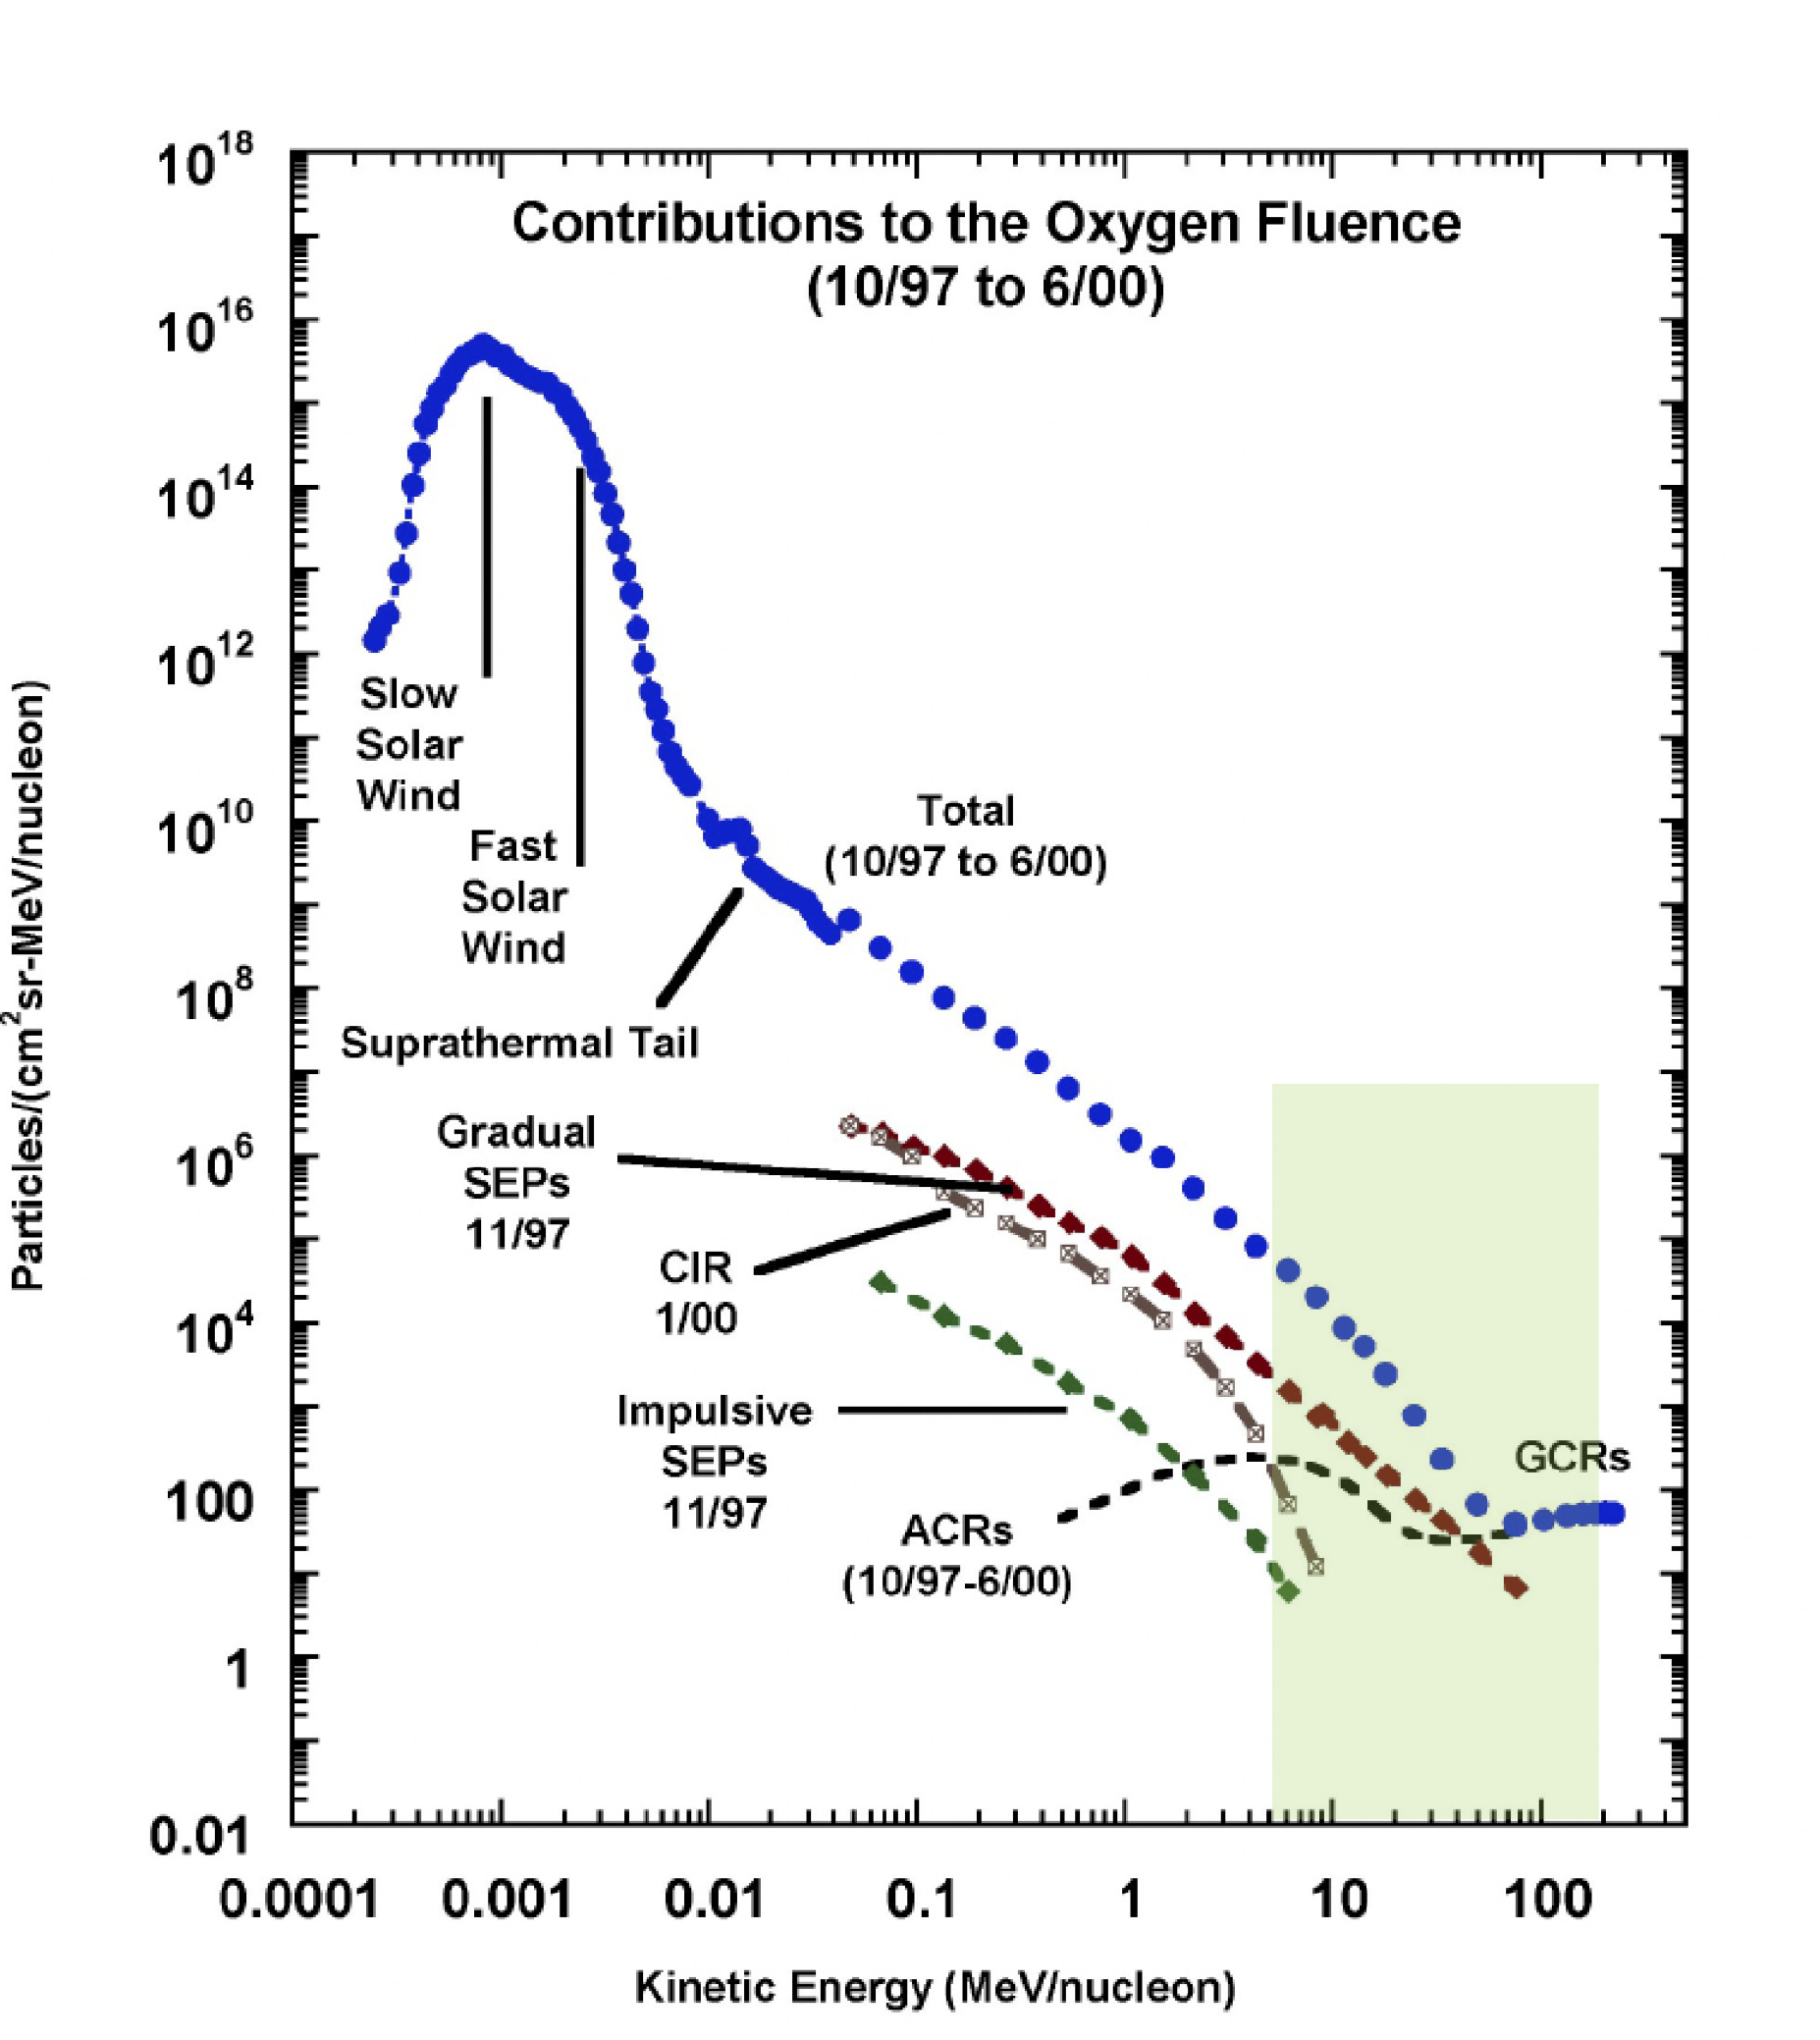
\includegraphics[width = \textwidth]{images/heliospheric_particle_spectra_color.png}
	\caption[Energy spectra of oxygen ions in the near Earth space]{The typical oxygen spectra in the interplanetary space near the Earth, indicating the contributions of different populations, especially in the energy range between few MeV\/nuc and few hundreds MeV\/nuc, where \acs{SEP}, \acs{ACR} and \acs{GCR} both exist. The spectra of other particles species for instance, helium and proton, have the similar shape but different flux level on corresponding energy region. The figure is adapted from \cite{Mewaldt-2001}}
	\label{Fig:Oxygen_spectra_heliosphere}
\end{figure}

Heliosphere is a vast, bubble-like region in the space that is surrounding the Sun. This region is moving in the \ac{ISM} with a speed of 25 km/s [citation]. Such a cavity is created by the sun and governd by its magnetic field and solar wind; a huge amount of plasmas of various particle populations fill this space. The particle populations could be identified from Fig.\ref{Fig:Oxygen_spectra_heliosphere} which is adapted from the measurements by \citet{Mewaldt-2001}. Based on the accumulated measurement of oxygen by \ac{ACE} between 1997 and 2000, the fluence oxygen spectrum which span over the energy range of more than 7 orders of magnitude from keV/nuc to GeV/nuc show clearly the lower energy particles including solar solar wind, fast solar wind,suprathermal tail, and high energy particles consist of \ac{SEP}, \ac{CIR}, \ac{ACR}, and the extremely high energy \ac{GCR}. 
Among them \acs{GCR} are from very distant source out of solar system, \acs{ACR} source are around the boundary of heliosphere, and the remain energetic particles are the parrticle accelerated and generated inside of the heliosphere at the locations including solar, interplanetary space and even the several planets of solar system for instance Jupiter.

Solar wind is a charged particles stream, also called plasma, released from the solar corona. Such a group of plasam consists of mainly protons and electrons that continously flow outward and expend to about $\sim$ 100 au (differ in the directions). The typical energy range of the solar wind is between 0.5 keV and 10 keV. Depending on the locations on the sun that produces the solar wind, the speed and density of solar wind might be different. For instance the fast solar wind with a typical speed between 500 and 800 kilemeters per second emits from the coronal holes which are funnel-like regions of open field lines in the magnetic field and usually appear in the north and south pole of sun. Therefore, the fast solar dominate the high latitude regions. While the slow solar wind is observed to have a velocity of about 300 - 500 kilometers per second and is believed to originate from the streamer belt along the equatorial belt. The slow solar wind is more likely to be observed in the low latitude regions.

%plasma embedding with magnetic field

Suprathermal particles are charged ions and electrons that move about two to hundreds times faster than the solar wind. In the spectrum shown in Fig.\ref{Fig:Oxygen_spectra_heliosphere}, the suprathermal particles are beyond the tails of the fast solar wind and are the dominate particles between few keV to hundreds of keV. The source of suprathermal particle might be the acceleration of solar wind and the remanent of the previous solar eruptions and \ac{SEP} events. Those particles play am important role in contributing seed particles for the \acl{SEP}	events.

Above the energy suprathermal particle are the energy range that we are interested in this thesis, especially the energy range between 10 MeV/nuc and few hundred MeV/nuc where the dominated particles are solar energetic particles (not limited to this energy range), anomalous cosmic rays (up to $\sim$ 100 MeV/nuc) and lower energy galactic cosmic rays. The new measurements in this study are from this energy range.

The \acl{SEP} are the high energetic particles with energy of few keV up to $\sim$ GeV oriented from the sun and accelerated during the solar activities like solar flare and \ac{CME} driven shocks. \acs{SEP} events are recurring, short term, but intensive. Different type of \acs{SEP} events persist different time scales, various from less than days to few days. Such high energy particles are one of the major threats in the space.
%also particle from solar, accelerated by different mechanism. The enery range of \ac{SEP} are quite broad, especially depending the on where the measurement carried on. Recently \ac{SOLO} and \ac{PSP} frequently measure the hundreds keV \ac{SEP}.

\acs{ACR} are the high energy interstellar pick-up ions [citaion] which are ionized neutral interstellar atoms generated by solar UV radiation after they move cross the boundary and enter the heliosphere. Those ionizing particle are then carried by the expanding solar wind to the outer boundary of helioesphere, where they are accelerated by the termination shock and then propagate inwards. The typcial species that have been observed are proton, helium, oxygen, nitrogen, iron, neon, etc. [citaion]

\ac{GCR} are the fully ionized particles that is accelerated at the so-called supernova remnants \cite{Blasi2013AARv2013} which are outside of the solar system and bombard Earth in a slowly varying and constant way. The complete GCR spectrum cover the energy from typical 1MeV \citet{Potgieter2013LRSP} to ZeV which is way beyond the energy range in Fig.~\ref{Fig:Oxygen_spectra_heliosphere}. The \acs{GCR} is comprised of about 89\% of hydrogen, 10\% of helium, 1\% of heavioer ions as well as electron, positron and antiprotons. 

After entering the heliosphere, the transport of both cosmic rays are controled by the \ac{HMF}, hence \ac{ACR} and \ac{GCR}'s temporal variaton is highly related with the solar activities and the so-called solar modulation, which are periodcally change in 11 and 22 year periods. 


\section{Solar energetic particles}

\subsection{Discovery of SEP and two types of SEPs}

The 

discovery of SEP and history of SEP, first SEP discovery and the  19 by who, GLE.

After the discovery of the first GLE events, the observation of the SEPs gradually move from the ground to the space, benefiting from the development of the human spacer explorations.



SEP are high energetic particle oriented from the solar surface and extend solar corona and. 
There are two major types of acceleration mechanisms that are believed to 
acceleration happened in two location, solar flare  and CME driven shock

The first on is magnetic reconnection
the other one is the CME driven shock.

Based on our current knowledged, it is widely accepted that the form is corresponding to the so-call impulsive event and the later corresponding to the graduale. This is the famous two paradim picture [citation]


\begin{figure}
	\centering
	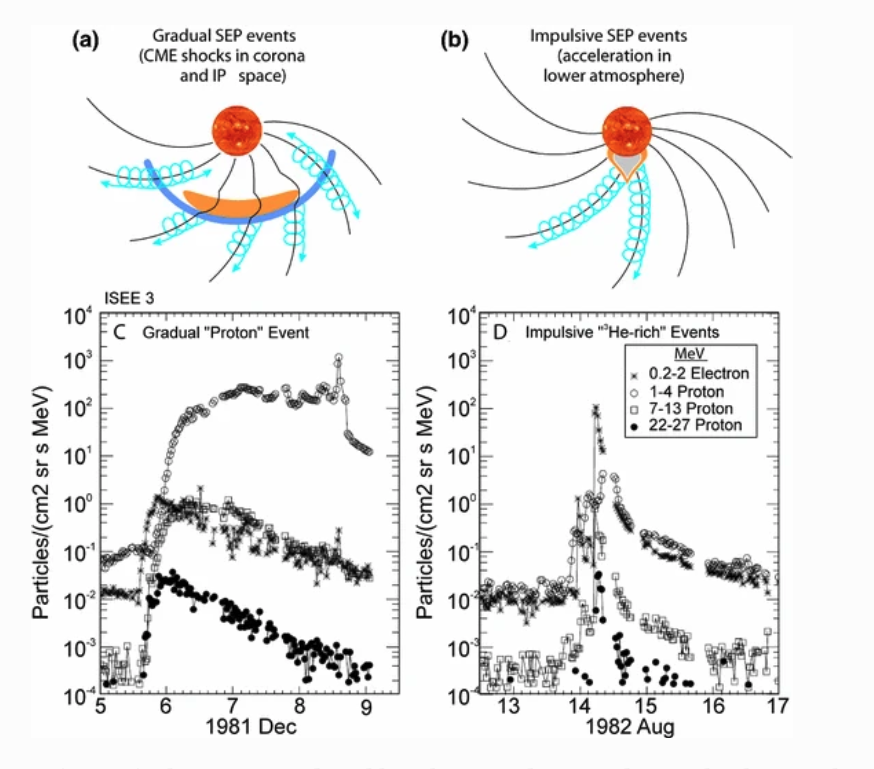
\includegraphics[width = 0.95\textwidth]{images/SEP_two_type.png}
	\caption[Two type of Solar energetic particle (SEP) event]{Two class of SEP events is presented. (a) The gradual SEP events that are associated with the CME drivens shocks in the coronal or in the interplanetary space and the particles populate the interplanetary magnetic field (IMF) lines over a wide range of longitudes. (b) The impulsive SEP event that is associated with the solar flares and the particles only populate a limited range of the open IMF lines that are well-connected to the flare site. Plots (c) and (d) are the corresonpding typical proton and electron time profile of the large gradual and small impulsive SEP events. The figure is reproduced from Desai \& Giacalone 2016}
	\label{Fig:two_type_SEP}
\end{figure}

Fig.~\ref{Fig:two_type_SEP} illustrate the current sceario of the two type SEP.

Find the corresponding paragraph and rephrase

\begin{itemize}
	\item Gradual SEP:
	\item Impulsive SEP::
\end{itemize}
Impulisve SEP: character; and special observation 

Gradual SEP: character; and 

A table that adapted from *** show the summary of the two type of SEPs

Apart from those distinct case, there is another type of \ac{SEP} which have the character of both impulsive and gradual. [what observations]
Such a event is call mix.

\subsection{Wide-spread SEP and Multiple instruments observation}

A numerous observation and simulation studies have been carried on in the past few decade since the discovery of SEP back to 1950s. The major questions of SEP focus on the origin, acceleration and transport of those high energy particles.\cite{Desai2016_review}, which is also the goal of recently two missions \ac{PSP} and \ac{SOLO}. 


Due to limited page allowance in the introduction part, we could not go through all those studies thoroughly. Instead, in this part we only focus on the so-called wide-spread SEP and the multiple instruments observation of SEP.
\begin{figure}
	\centering
	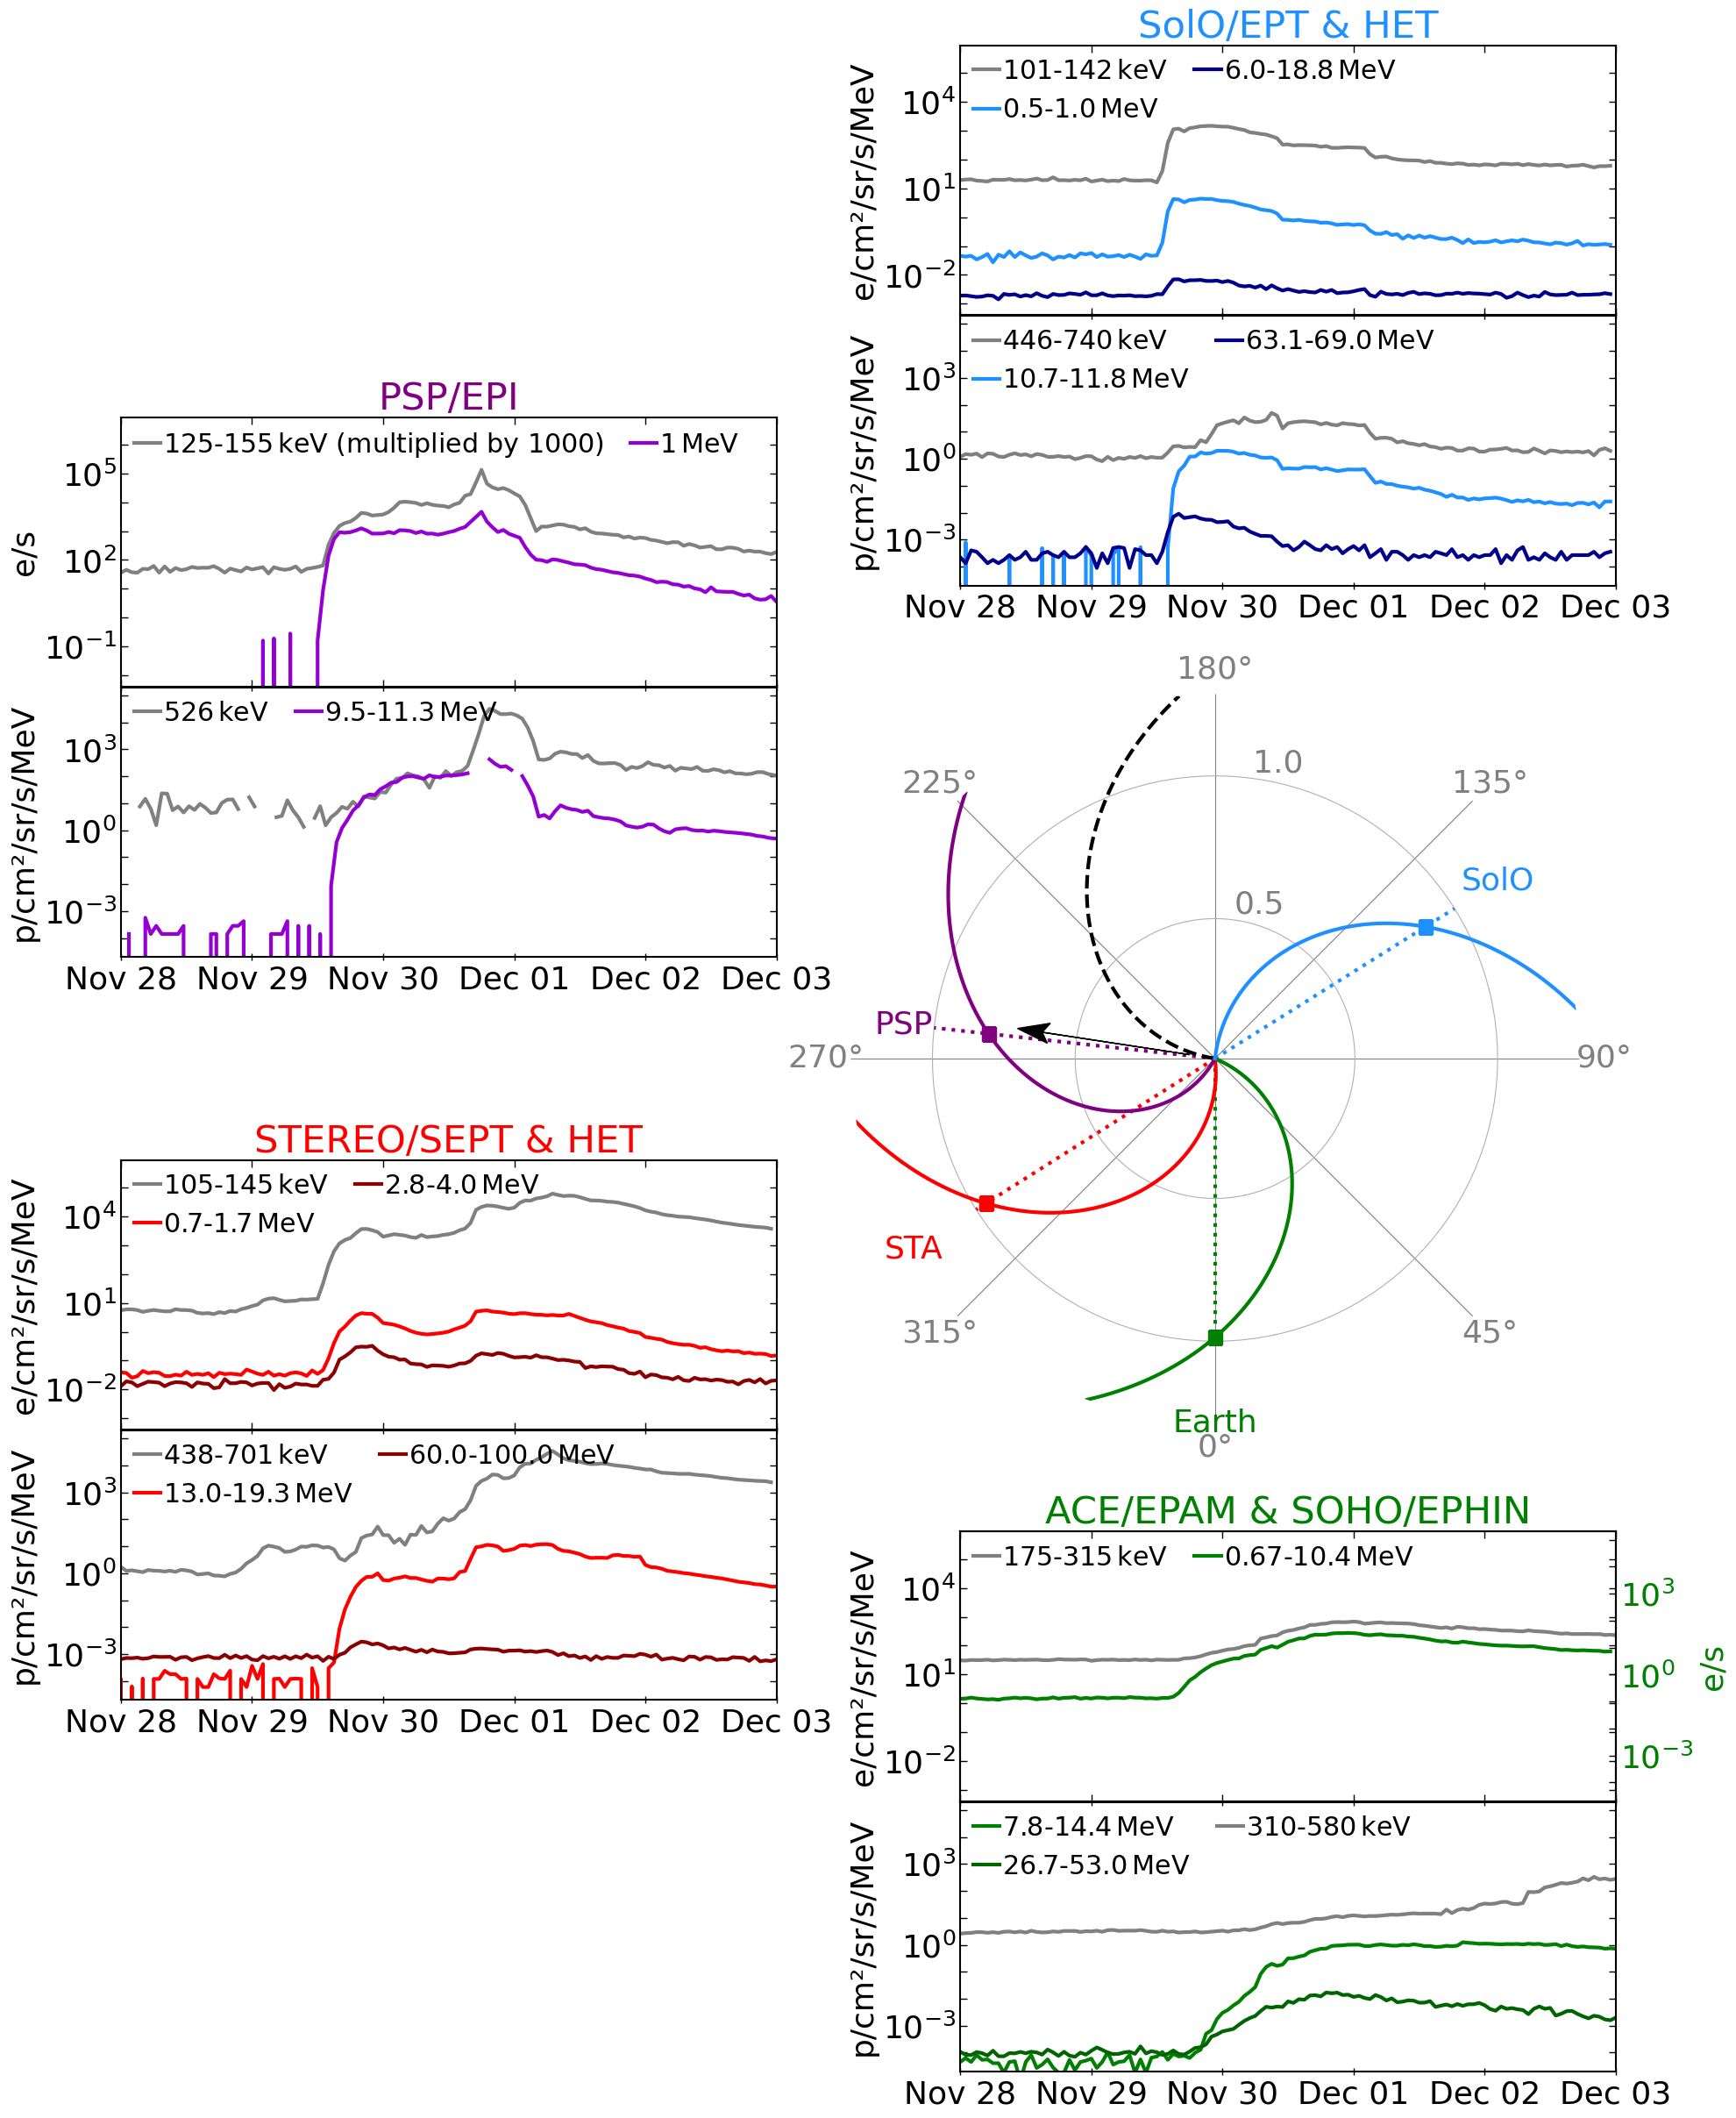
\includegraphics[width = \textwidth]{images/2020-11-29_overview_plot.png}
	\caption{The first wide-spread \acl{SEP} event on Nov 29, 2020. The figure is from \citep{Kollhoff-2021}}
	\label{Fig:SEP_widespread}
\end{figure}

Figure \ref{Fig:SEP_widespread} is the first widespread SEP of the SC 25. what paper

Wide spread SEP reflect the large longitudianl extend of the SEP.

What is wide spread SEP
What are the previous observation of wide spread, - ? gradual? - related information?

The major question is how the energetic particle spread the heliosphere.

The multiple obseravtion provide unique information - bring new information

Study both in-situ and remote.
Now - \ac{SOLO} \ac{PSP} and \ac{Bepi},  MarsSTEREO missson, helios mission, new mission from China, \citet{Wang2020Solarring,}India
together with 
Multiple instruments observation of wide-spread SEP provide unique opportunity to study the acceleration, release, and propagation of SEP in the heliosphere.



\section{Galactic cosmic rays} ( 1500 words are enough, 50 citation)

\begin{figure}
	\centering
	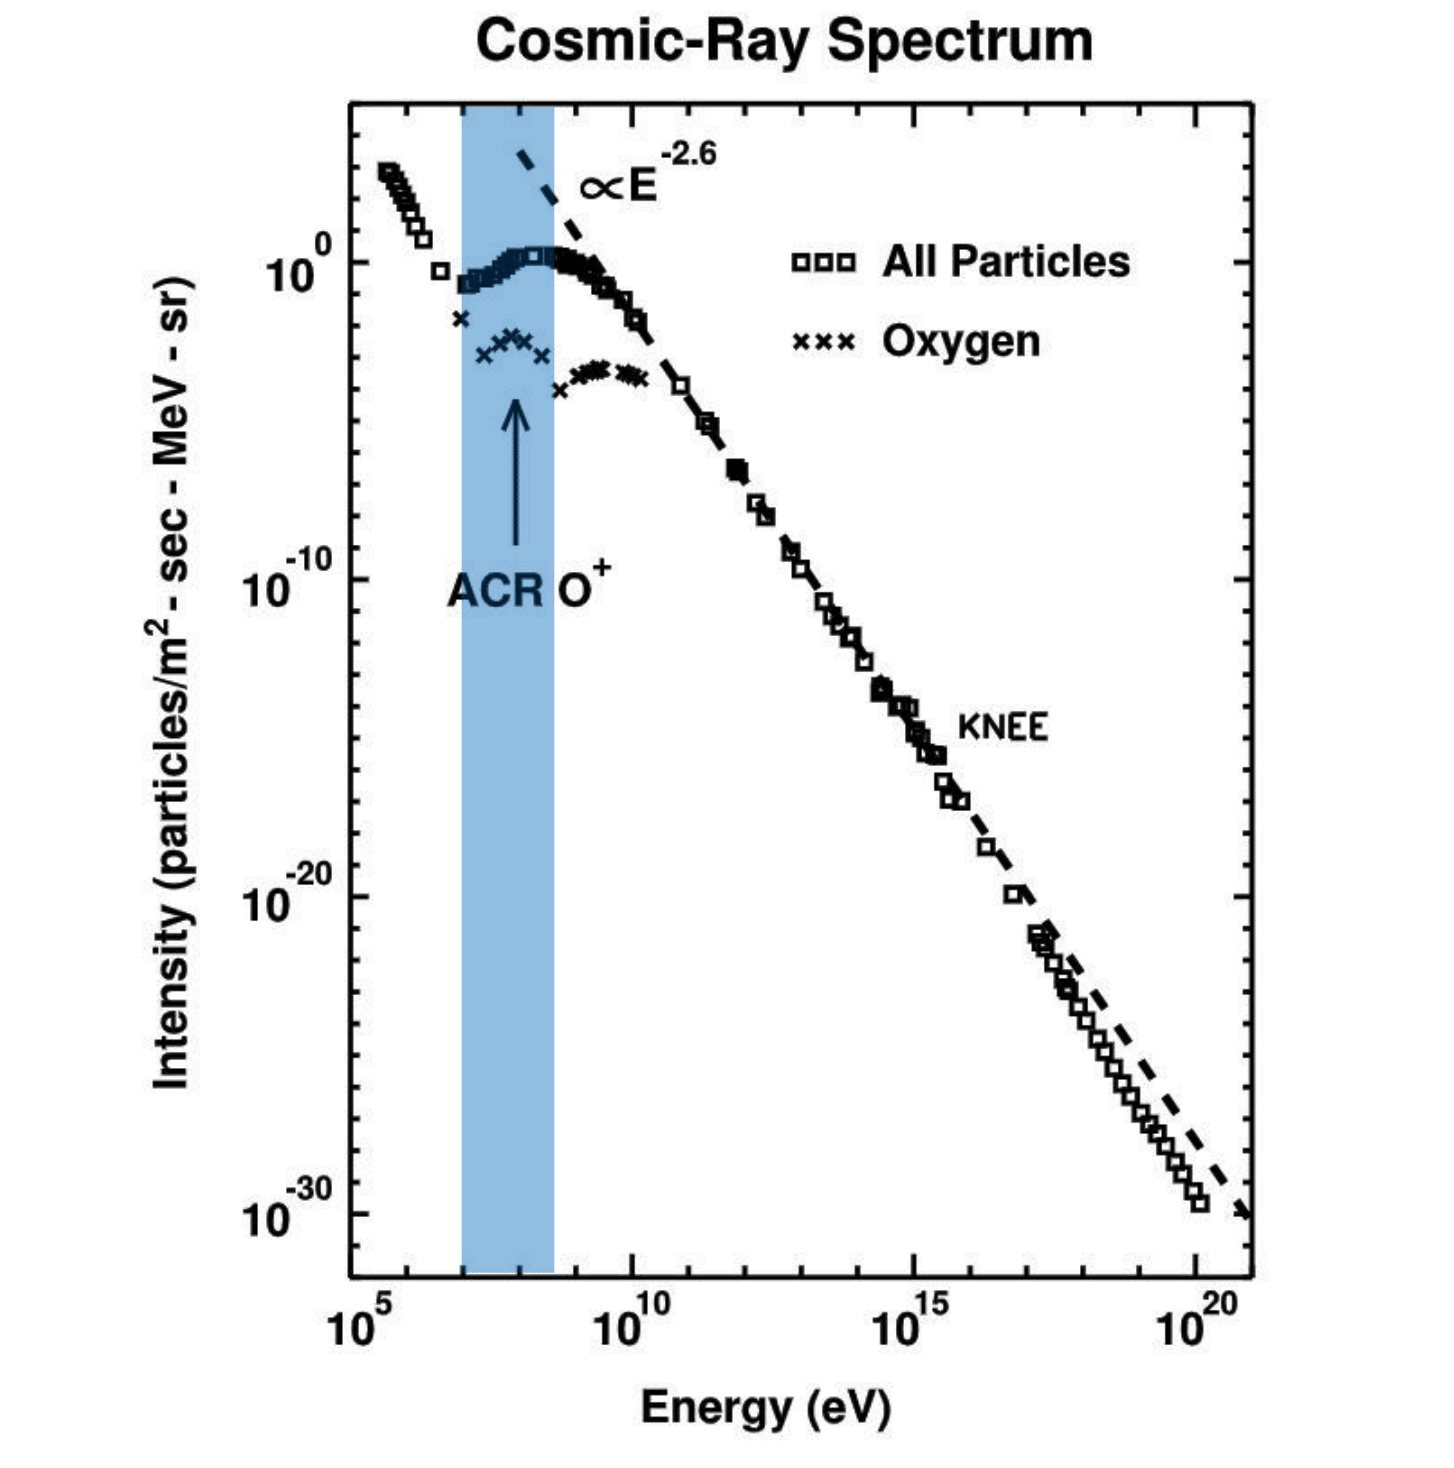
\includegraphics[width = 0.9\textwidth]{images/gcr_spectra_shadow.png}
	
	\caption{The cosmic spectra of all particles and ACR oxygens observed at 1 AU. This figure is from Giacalone 2021, 2012, and originally from Jokipii 1990.
	The spectrum is plotted in more than 15 orders of magnitude on the energy scale and about 30 orders of magnitude on the intensity scale, extend the high energy end of Fig.\ref{Fig:Oxygen_spectra_heliosphere}.}
	\label{Fig:Oxygen_spectra_cosmic_ray}
\end{figure}
%\url{https://timeline.web.cern.ch/victor-hess-discovers-cosmic-rays-0}
The first discovery of the galactic cosmic rays was made by the Victor Hess in 1912 when he carried on a ballon experiement. The initial purpose of the experiement was to find the source of ionizing radiation in Earth's atmosphere using the electroscope. However, as the ballon climb-up during the experiment, he found that ionization rate measured in the electroscope showed less signicant decrease than anticipated. Such a discrepancy was attributed to the existence of the cosmic rays which increase the radiation in the atmoshphere.

In figure \ref{Fig:Oxyge_spectra_cosmic_ray}, the full spectrum of the all cosmic particles observed at 1 AU which includes both the \ac{ACR} and \ac{GCR} components is shown. The \acs{GCR} are indicated as empty squares. In the right half of the spectra with energy above 1 GeV, the spectrum could be simply fitted by power a law spectrum with index of about -2.6. The knee of GCR spectra are around [] energy and reflect what mechanism[citation]. The lower energy spectrum is shown as a "turn over" below 1 GeV which are more complicated and could not be fitted by a signel power law. 

\acs{GCR} consist of multiple energetic particle species span a wide range of energy, which are mostly dominated by the proton, about 89\%  and the remains are shared by 10\% helium and a small portal of heavier ions (1\%), electron, positron and antiproton. 
It is believed that \acs{GCR} are mainly originated from the supernova remanent very far from the sun[citation] and obtain the energy from the shock waves which is genereated from the explosion of supernova. When the shock wave travel through the surrounding interstellar gas, the kinetic energy of shock are tranfer to the  (neutral gas?) by the (Fermi-acceleration, ciataion and the acceleration process), Utilimatly, the energetic particle with energy up to 10$^12$ eV are created.
After a long travel, \acp{GCR} arrived the local bubble controled by the sun and its magnetic field. Before entering the heliosphere,  the particles are isotropic distributed in space and nearly constant  in time. Because cosmic rays are fully charged, they are deflected by the magnetic field when they propagation in the interstellar space after speeding up. The directions of those particle are normalized by the strong magnetic field. Hence when they arrived at the local bubble of solar system, we obtained an nearly isotropic and constant intensity profile [citaion of the LSTM,]

To model the solar modulation on the particle transportation of GCR spectra, an input particle spectra need to be specifield, which is the so-call LSTM [ citaion of LSTM]. LSTM is the modulation boundary and will be modulatined as the change of the position, energy, and time after those particle diffusion into the heliosphere. Such a spectra have been observed by the voyeger after then cross the boundary of solar system and enter the interstellar medium.

% As shown in the Fig.\ref{Fig:Oxygen_spectra_heliosphere}, the dominated energy of \acs{GCR} is above 100MeV/nuc.  
% ---- To do
% [Describe the GCR spectra]
% Below that, the other component are more common than GCR and it is hard to seperated those particles.
%  ---
%A paragraph of local intersteallar spectra ?

After enter the heliosphere, those high energetic particle are modulated the solar wind and its embedding magnetic field  which changes in a 11 year or 22 year period, which is so-called solar cycle.
The relavant process of the solar modulations could be described by a basic transport equation (TPE) which is first derived by Parker (1965). The same equations was also derived by Gleeson and Axford (1967) in the more rigorous ways. This equation is based on the motion of charged and particle in the high frequently changed magnetic field and averages over the pitch angle of particle moving in the magnetic field. The precondition of this equation is the reasonable assumption of the isotropically distributed GCRs. The TPE give the phase-space distribution function, $f$ as the function of positions, time and momentum magnetitude. In Potgieter (2013), the helispheric TPE, based on Parker (1965) is rewritten in the following form:

	\begin{equation}
		\underbrace{\frac{\partial f}{\partial t}}_{a} = - ( \underbrace{\boldsymbol{V}}_{b} + \underbrace{\langle v_d \rangle }_{b}) \cdot \nabla f + \underbrace{\nabla \cdot (\boldsymbol{K_s \cdot \nabla f})}_{d} + \underbrace{\frac{1}{3}(\nabla \cdot \boldsymbol{V}) \frac{\partial f}{\partial ln P}}_{d}
		\label{Eq:Transportation_equation}
	\end{equation}

where $f(r, P, t)$ is the cosmic ray distribution as the function of the time t, particle rigidity P and 3-dimension position in the space. Compared with the $\sim$ 11 years solar cycle, the periodcally solar rotation ($\sim$ 27 days) and  the time of the solar wind traveling to the edge of helipshere ($\sim$ 1 years) are short-term variation and can be neglected. Hence the steady-state solution with  $\frac{\partial f}{\partial t} = 0$ (part a of Eq.\ref{Eq:Transportation_equation}) is a reasonable assumption and also considered. Terms in the right parts include four effects that are used to describe the variation of the cosmic rays: (b) convection due to the solar wind velocity $\boldsymbol{V}$; (c) drift effects caused by the gradient and curvature of the large-scale \ac{HMF}, which is estimated by a 3D Archimedean spiral (Parker 1978), $\langle v_d \rangle$ represents the averaged drift velocity; (d) diffusion effects caused by the turbulent mangetic field, with the $\boldsymbol{K}_s$ the symmetrical diffusion tenser; (e)adiabatic energy change and deceleration due to the expansion of the solar wind. 

Since TPE is a high non-linear partial differential equation, only a simplified solution of the GCR spectra is derived which is called the Force-field Solution (FFS). The FFS was first derived by Gleeson and Axford [1967, 1968b], which simply depend on the kinetic energy T of particles and the solar modu. Later, a reasonable GCR spectra of the particle with energy above 150 MeV were given by Gleeson and Urch 1973.
With the development of computer technque and numerical studies, simulation are becoming more and more important in studying the tranporation and solar modulation of the cosmic rays. [Jokippi and Kopriva 1979, Le Roux and Potgieter 1995, Manuel et al 2011, and Potgieter 2013, Vos \& Potgieter 2015, 2016; Boschini et al. 2019;
Corti et al. 2019; Shen et al. 2019 \url{https://iopscience.iop.org/article/10.3847/2041-8213/acbea7/pdf}]. 
Several popular used model like BON14, 2020, CREME 96 and HELMOD based the solar modulation and sunspot numbers could easily reproduce the GCR intemnsity and spectra which are consistent with the measurements from \ac{ACE} in 1 AU and Voyager probes in the different regions of helisophere [Boschini et al 2019- Model]

\begin{figure}
	\centering
	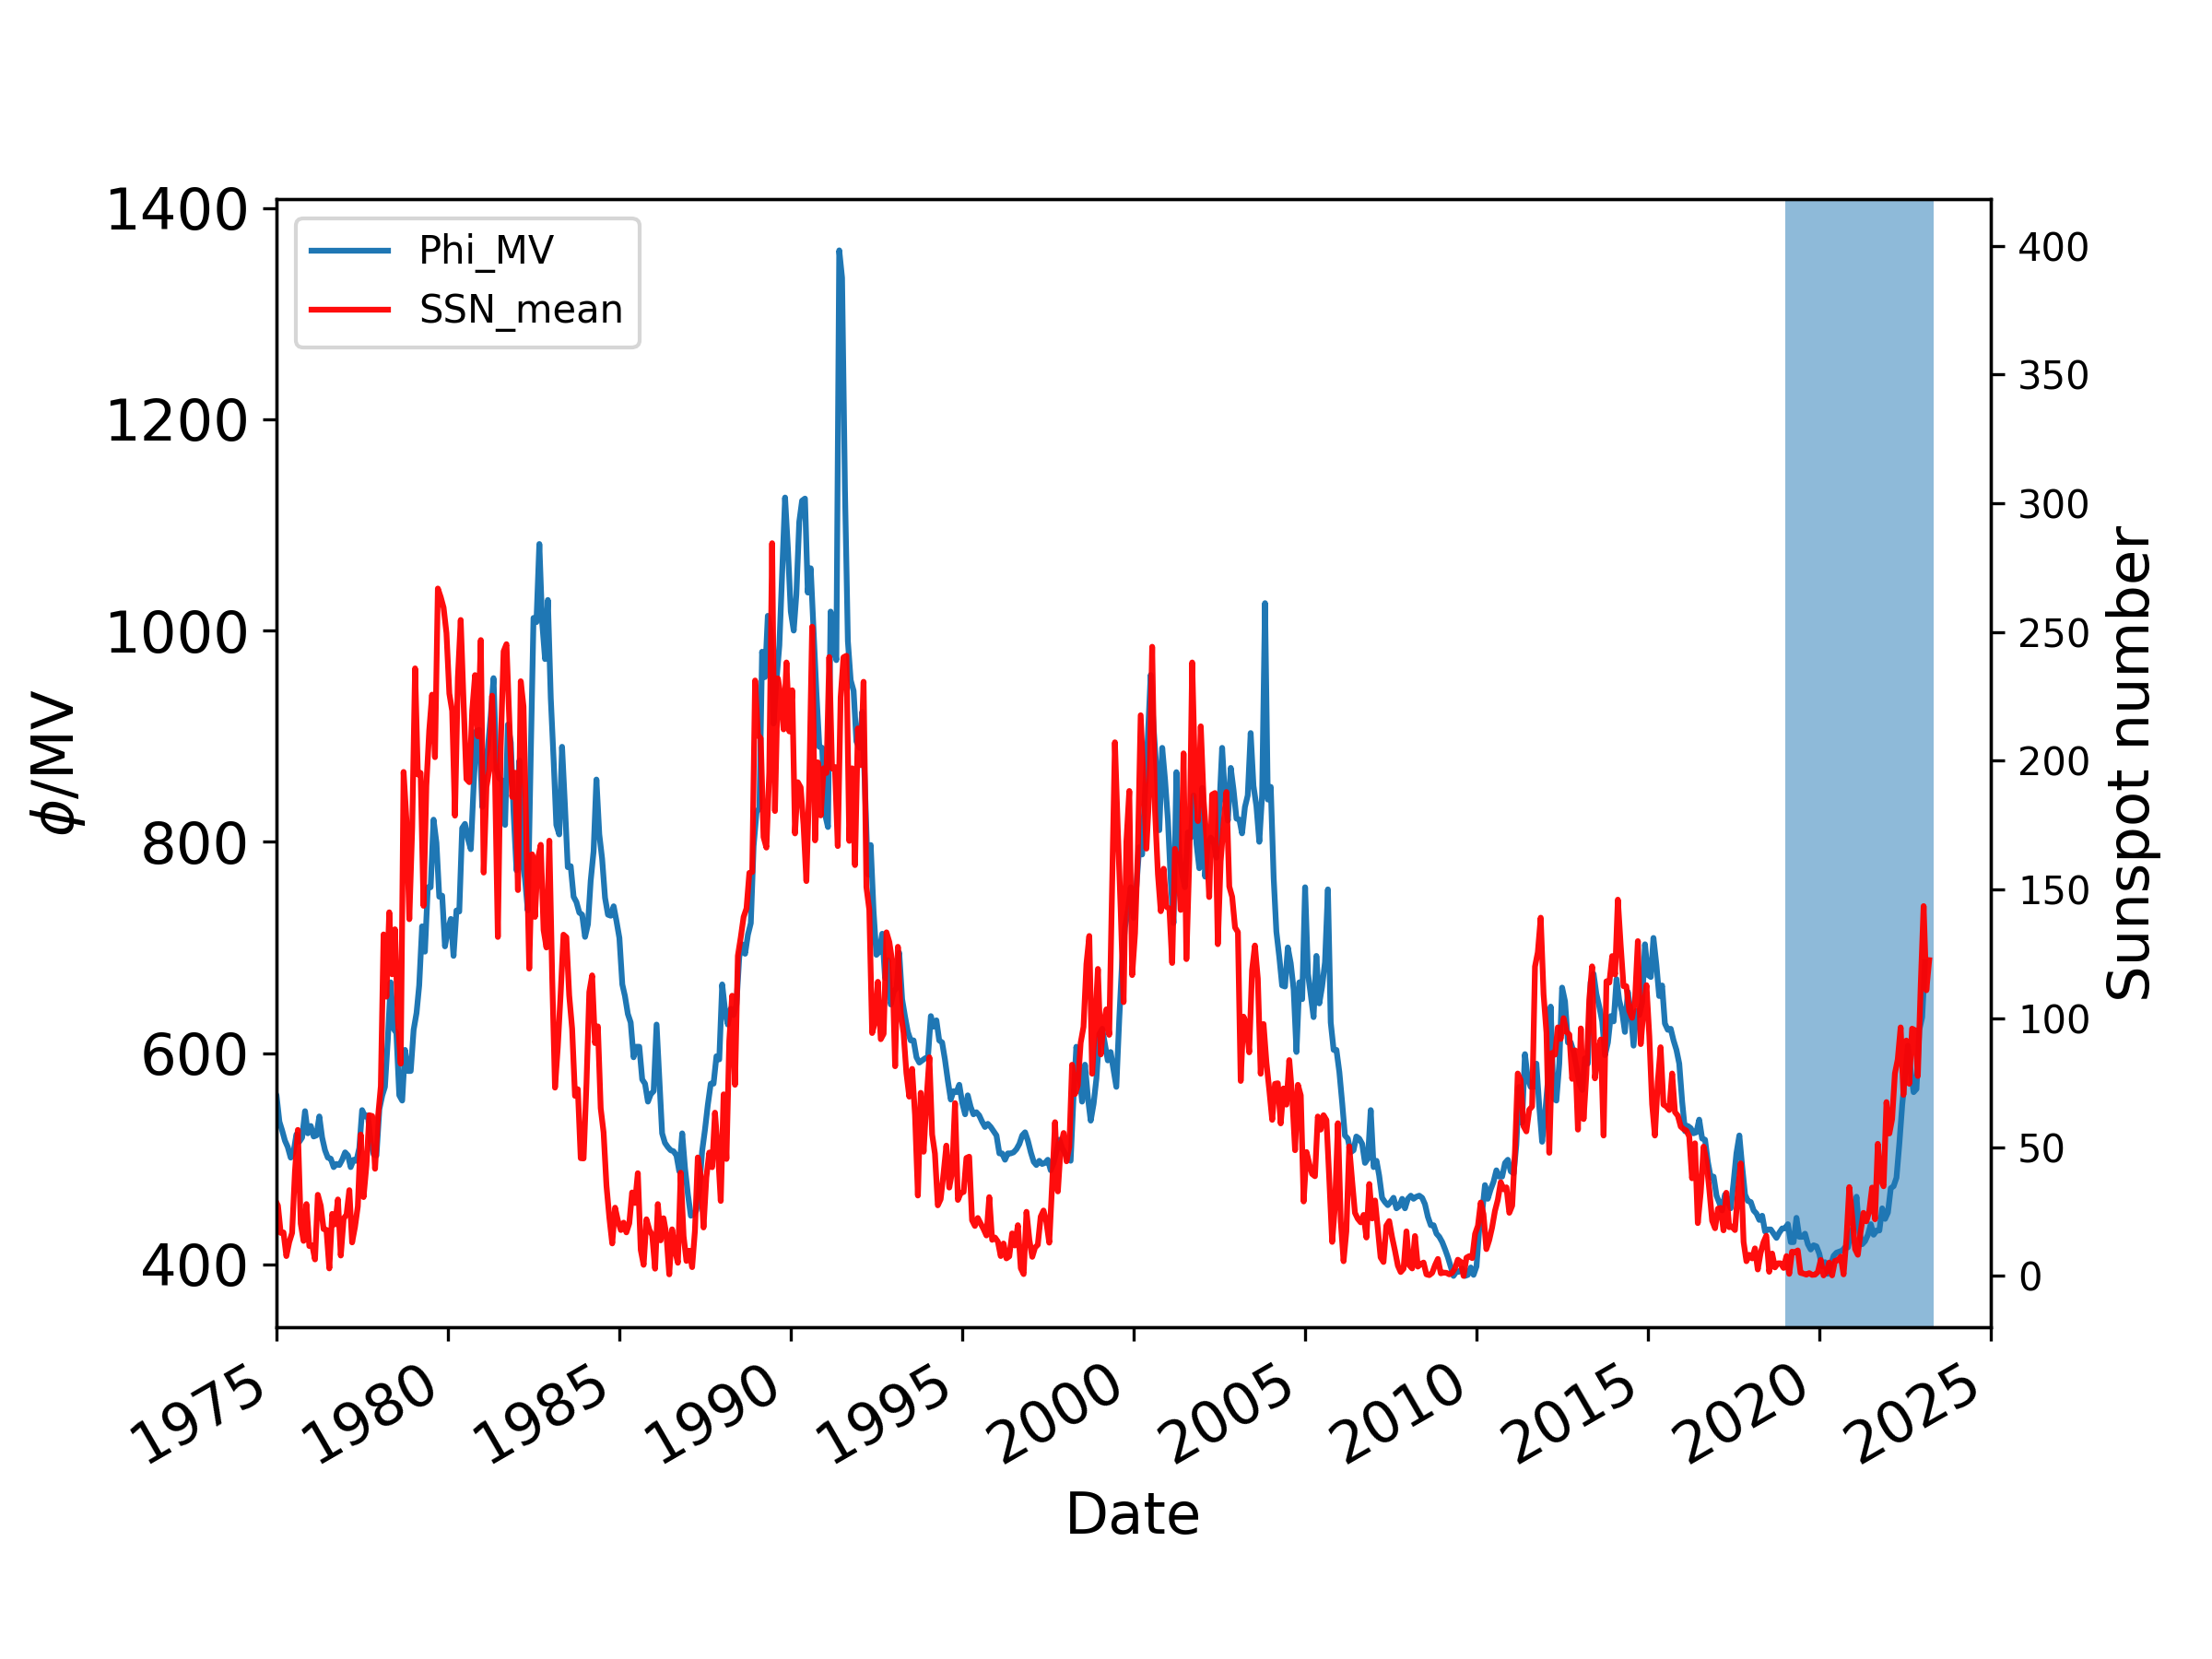
\includegraphics[width = 0.9\textwidth]{images/Solar_modulation.png}
	\caption{The solar modulation potential ($\phi$) \cite{Usoskin 2011}, data are downloaded from \url{https://cosmicrays.oulu.fi/phi/phi.html}, and the monthly averaged sunspot number from Solar Influences Data analysis Center (SIDC), Royal Observatory of Belgium, Brussels, \url{https://www.sidc.be/silso/datafiles}}
	\label{Fig:Solar_modulation}
\end{figure}


Figure \ref{Fig:Solar_modulation} show the monthly averaged sunspot number since 1975 in red and the solar modulation potential ($\phi$) \cite{Usoskin 2011}.
Sunspot number is a proxy for the solar activities. The variation of the solar modulation potential align with the variation of solar activities in the solar cycle.
The GCR flux is anti-correlated with the averaged sunspot number, that is the GCR flux peaks when the sunspot number is minimum during solar minimum and vice versa in the solar maximum.
The time between two neighbouring solar minimum is about 11 years, which is the period of the solar cycle and caused by the polarity reversal of the solar magnetic field, which is the solar cycle.

Besides the magnetic field reversal, the drift effects play an important role in the 22-year cycle of the intensity of cosmic rays. Such effects are clearly observed in the temperoal variations.
As shown in Fig.\ref{Fig:Solar_modulation}, during the A < 0 cycle, GCR had a more peaked time profile than A > 0 cycle, which have a plateau-like profile. 
This because in the A < 0 magnetic polarity cycle, the positively (negatively) charged particles drift inwards (outwards) mainly along the equatuorial plane in the heliosphere and drift outward (inwards) through the open mangentic field in the polar region, resulted the sharp change of the intensity. While in the A > 0 cycle, the drift direction of the particle is opposite to the A < 0 cycle, caused the plateau region on the solar minimum. Fig.~\ref{Fig:drift_effect} illustrate the drift effects in the opposite polarity cycles, showing the drift directions of the positively charged particles like helium, oxygen.

\begin{figure}
	\centering
	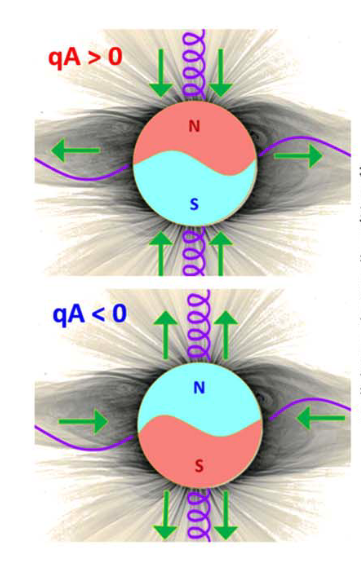
\includegraphics[width = 0.5\textwidth]{images/drift_effect.png}
	\caption{The illustration of the drift effects, adapted from the Fig. 4 of \citep{Rankim 2020?}}
	\label{Fig:drift_effect}	
\end{figure}

Furthermore, the drift effects are also reflected in the spatial gradient [Vos and Potgieter 2016] of the cosmic rays. 
\TODO{add more here}
The spatial gradient, including the latitude and radial gradients have already been observed by multiple missions for the region from 1 AU to the edge of the heliosphere in the past few solar cycles, for instance the two Voyager probes, the Ulysses spacecraft, Pioneer and also combined the measurements like PAMELA from L1 point, [citaion]
Besides, the charge sign-dependent radial gradients have been measured, finding the positive and negative latitude gradients in the outer helisphere. [citaion]
The GCR spatial gradient have not been studied in following chapter but will be studies in future base on the new measurement of the PSP and SOLO missions.

As ** indicating the solar minimum of SC 23/24 was quite unusual, with a much weaker \ac{HMF} compared with the history record and a higher then ever GCRn intensity. Further more, The recent solar minimum 
is even more unusual, the highest GCR intensity in the history and the unusual ACR intensity [that paper]. 


Therefore, the studies of both the temperal variation and spatial gradient are still not compeleted and it is still worthwhile to check the GCR data with more new data and by more detailed analysis.

	


\section{Anomalous Cosmic Ray}

Anomalous cosmic rays are mostly the singly charged energetic particle dominated the energy range between few meV/nuc to $\sim$ 100 MeV/nuc. \acs{ACR} were firstly discovered by the \acs{IMP} 7 and 8 in 1970s [citation]. By analyzing the lower spectra of cosmic rays, [who] et al found an "unusual" enhancement of the flux of [particle species]. As the oxygen spectra in Figure \ref{Fig:Oxygen_spectra_cosmic_ray}, the intensity of oxygen did not decrease as the energy decrease from hundred MeV/nuc to MeV/nuc, but incrase
Currently, both ACR helium, oxygen, neon, protons have been found in the outside of 1 AU region and what find in 1 AU

It is believe that ACRs are the high energy interstellare pick up ions which are accelerated in termination shock of the heliosphere. Extend this to a paragraph;
The possible acceleration mechanisam of the ACR include  (citaion)

One of the key chararcters of ACR is that those energy particles are singly charged, which could help use to seperate the ACR from the GCR and SEPs. [Find a paragraph to extend the charge state analysis] - a relatively detailed observation history of the ACR charge state which is already the fixed answer. - Explain.

Though the source of ACR and GCR are total different, after they entering the heliosphere, the energetic particles endourver the same transport process and interact with the solar wind and magnetic field,  which together could be described by the TPE equation.

By 1 AU, similar to GCR intensity, ACR intensities are also heaviely modulated during their transportation in the solar wind and globar \ac{HMF}. Figure \ref{Fig:ACR_solarmodulation} show the comparison between the ACR oxygen intensity and the neutron monitor count rate which is a proxy of the GCR variation in the deep space. The peaked and plateau-shaped profiles in the last two and half solar cycles are consistent in two measurements.


\begin{figure}
	\centering
	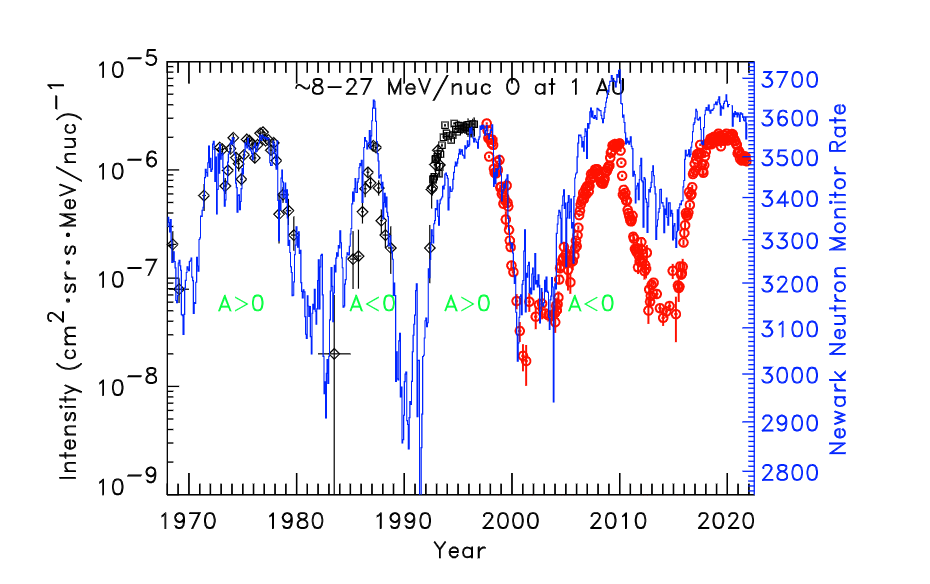
\includegraphics[width = 0.9\textwidth]{images/ACR_solarmodulation.png}
	\caption{ACR oxygen intensity with energy between 8 and 27 MeV/nuc at 1 AU measured by ACE/SIS instrument (red) and count rate of Newark Neutron monitor (blue). The plot is adapted from Figure 6 of Giacalone et al 2022}
	\label{Fig:ACR_solarmodulation}
\end{figure}

The spatial gradient consist the important information of the transportation and acceleration of the ACRs in the heliosphere and in the terminaton shock \cite{Rankin 2020}. 
The radial and latitude gradient of ACR in the region outside of 1AU

Below 1 AU, Marqunet, Helios, number 
And more recently, Rankin, PSP, find Oxygen and protons

\section{Radiation hazard of energetic particle}

Studying the radiation hazard of the energetic particles are of great importance to the human exporation activities.
The radiation include the SEP caused short time but intensive radiation
GCR cause the long-last radiation which is less intensive but still harmful to the human body, especially during the solar minimum when the flux of GCR peaked.

The hazard of energetic particle 

Energy range - LND instrument paper

\begin{figure}
	\centering
	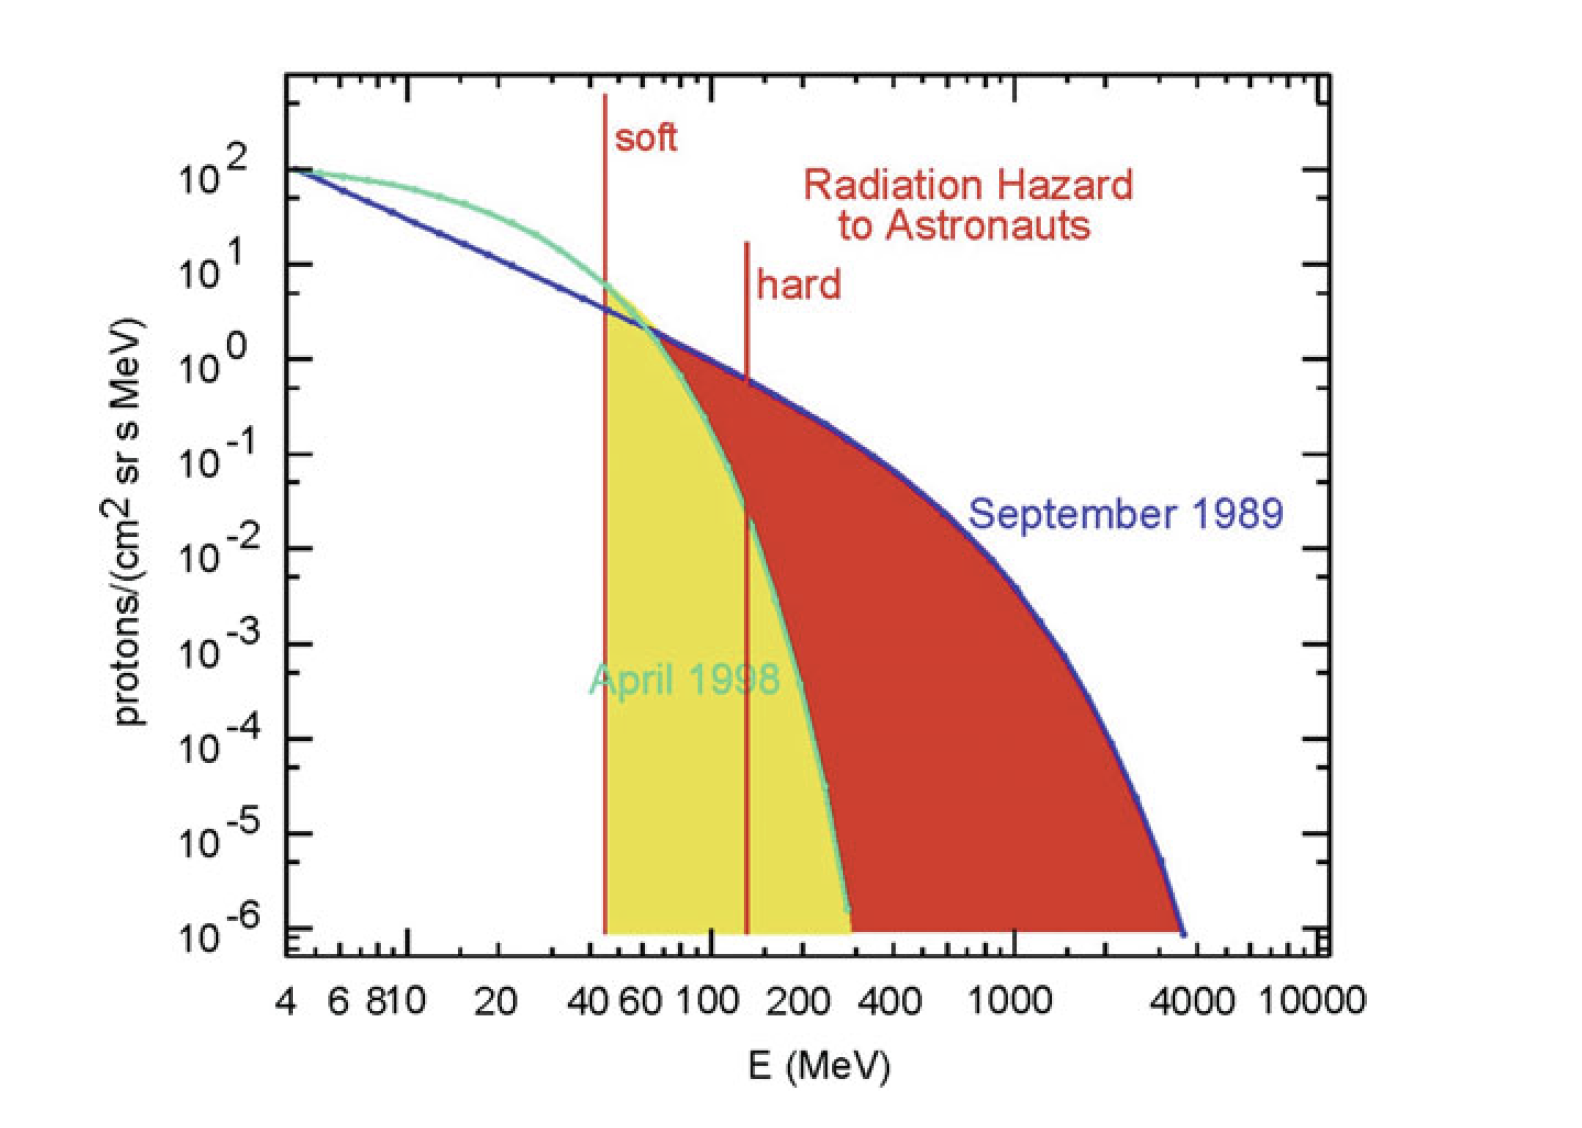
\includegraphics[width = 0.6\textwidth]{images/SEP-radiation_hazard.png}
	\caption{The protons spectra of two SEP events. The shadow regions indicates the harmful energy of the protons. Different spectra types - hard and soft - both threathen the human activities. The figure is adapted from Reames 2021 [textbook]}
	\label{Fig:SEP-radiation_hazard}
\end{figure}
Radiation hazard of the SEP 


\begin{figure}
	\centering
	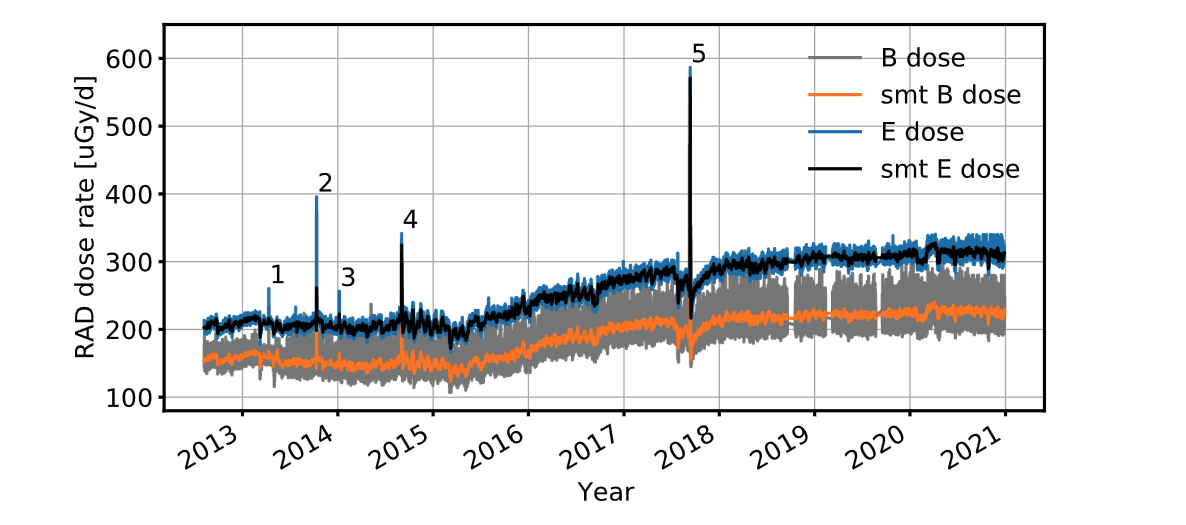
\includegraphics[width = 0.9\textwidth]{images/Rad_GCR_radiation.png}

	\caption{The radiation dose rates on the Martian surface, measured by the \ac{RAD} in the silicon detector B (grey) and plastic detector E (blue). The daily averaged dose rates of B (smt B dose, orange) and E (smt E dose, grey) overlay the original measurements. Apart from 5 prominent SEPs (number 1-5), the long-term trend of dose rate is correlated with the \ac{GCR} variation. The figure is reproduced from \citep{Guo2021AARv_rad}}
	\label{Fig:Rad_GCR_radiation}
\end{figure}
	
Apart from the primary radiation from the GCR, which is modulated by t

- GCR interaction with regolith, lunar-
	- Generation of Neutron

The exploration of space has witnessed a surge in intensity, with an increasing number of countries aspiring to venture into this domain. Noteworthy examples include NASA's initiation of the Artemis mission, which aims to return to the Moon by 2024. Similarly, China has unveiled its plans to establish a lunar base on the lunar surface by the 2030s, while the European Space Agency (ESA) has also embarked on a lunar lander mission. Most recently, a Japanese lunar lander mission was launched; however, it regrettably encountered failure.

Under these circumstances, the study of solar energetic particles (SEPs) assumes greater significance. SEPs pose a significant radiation hazard for future human exploration on the lunar surface. The most hazardous SEP events have the potential to induce radiation increases of substantial magnitude.

\subsection{Motivition}

The few tens of MeV energy range is an very important energy range for the heliosphere. In this part the SEP, ACR, lower GCR are bothe there. Therefore, more attention required here

New measurements, new time and multipoints (NNM)
new age (deep space age)

New instrument, new data, PSP launched, SOLO, LND, and many other missions of different goverment
Such new observation provide valuable data to study the energetic particles
Secondly, as we described above, the solar minimum of SC 23/24 is unusual, and the recent solar minimum is even more unusual, the highest GCR intensity in the history and the unusual ACR intensity [that paper]. Such unusual solar minimum provide a good chance to study the solar modulation of the energetic particles. Special Solar minimum
Furthermore, the radiation hazard of high energy particle is of great interests to the human space exploration. 


Therefore in the following section of the thesis, following the idea of using the totally new measurements from SOLO and LND, we will show the new observation of SEP from the LND, GCR and secondary proton measurement on the Luanr surface, quite time spectra (GCR) measure in the inner heliosphere and the radial gradient change of the ACR helium in the new solar cycles.